\documentclass{article}

\usepackage{upquote,natbib,graphicx,amsmath}

\begin{document}

\title{An algorithm for U--Pb geochronology by secondary ion mass spectrometry}

\author{Pieter Vermeesch\\
  London Geochronology Centre\\
  Department of Earth Sciences\\
  University College London\\
  London WC1E 6BT\\
  United Kingdom\\~\\
  \texttt{p.vermeesch[at]ucl.ac.uk}
}

\maketitle

\begin{abstract}
  Secondary Ion Mass Spectrometry (SIMS) is a widely used technique
  for in-situ U--Pb geochronology of accessory minerals. Existing
  algorithms for SIMS data reduction and error propagation make a
  number of simplifying assumptions that degrade the precision and
  accuracy of the resulting U--Pb dates. This paper uses an entirely
  new approach to SIMS data processing that introduces the following
  improvements over previous algorithms. First, it treats SIMS
  measurements as compositional data, using logratio statistics. This
  means that, unlike existing algorithms: (a) its isotopic ratio
  estimates are guaranteed to be strictly positive numbers; (b)
  identical results are obtained regardless of whether data are
  processed as normal ratios
  (e.g. \textsuperscript{206}Pb/\textsuperscript{238}U) or reciprocal
  ratios (e.g. \textsuperscript{238}U/\textsuperscript{206}Pb); and
  (c) its uncertainty estimates account for the positive skewness of
  measured isotopic ratio distributions. Second, the new algorithm
  accounts for the Poisson noise that characterises Secondary Electron
  Multiplier (SEM) detectors. By fitting the SEM signals using the
  method of maximum likelihood, it naturally handles low intensity ion
  beams, in which zero-count signals are common. Third, the new
  algorithm casts the data reduction process in a matrix format, and
  thereby captures all sources of systematic uncertainty.  These
  include significant inter-spot error correlations that arise from
  the Pb/U--UO\textsubscript{(2)}/U calibration curve.  The new
  algorithm has been implemented in a new software package called
  \texttt{simplex}. \texttt{simplex} was written in \texttt{R} and can
  be used either online, offline or from the command line. The program
  can handle SIMS data from both Cameca and SHRIMP instruments.
\end{abstract}


%\copyrightstatement{TEXT} %% This section is optional and can be used for copyright transfers.


\section{Introduction}  %% \introduction[modified heading if necessary]

Secondary Ion Mass Spectrometry (SIMS) combines high sensitivity with
high mass resolution \citep{williams1998}. This allows the technique
to obtain precise U--Pb dates on ng-sized samples whilst resolving
isobaric interferences on \textsuperscript{204}Pb to a degree that is
currently unachievable by other techniques such as Laser Ablation
Inductively Coupled Plasma Mass Spectrometry (LAICPMS).  There are
some other differences between LAICPMS and SIMS as well. LAICPMS
instrumentation is built by numerous manufacturers, whose data files
are compatible with a rich ecosystem of data reduction codes such as
\texttt{Iolite}, \texttt{Glitter} and \texttt{LADR}.  This facilitates
the intercomparison of different laboratories, different instrument
designs and so forth.  In contrast, the SIMS U--Pb world is dominated
by just two manufacturers, whose SHRIMP (Sensitive High Resolution Ion
Micro-Probe) and Cameca instruments use completely separate data
reduction protocols. Most SHRIMP laboratories use \texttt{Squid}
\citep{ludwig2000,bodorkos2020}, which is incompatible with Cameca
data.  In contrast, Cameca data tends to be processed by in-house
software such as M. J. Whitehouse's NordSIM spreadsheet, which are
incompatible with SHRIMP data.\medskip

This paper introduces a unified algorithm for SIMS U--Pb data
reduction that aims to address five problems with existing data
reduction methods. The first three of these problems are:

\begin{enumerate}
\item Accuracy: existing algorithms give (slightly) different results
  depending on whether the raw data are processed as
  \textsuperscript{206}Pb/\textsuperscript{238}U-ratios or as
  \textsuperscript{238}U/\textsuperscript{206}Pb-ratios,
  say. \label{it:accuracy}
\item Precision: current data reduction routines produce symmetric
  confidence intervals, which are unrealistic for low intensity ion
  beams. \label{it:precision}
\item Systematic uncertainties: current data reduction protocols use a
  hierarchical error propagation approach, in which random
  uncertainties and systematic uncertainties are propagated
  separately. However such a clean separation is not always possible,
  and this can complicate higher order data processing steps such as
  isochron regression and averaging. \label{it:syserr}
\end{enumerate}

Sections~\ref{sec:accuracy} -- \ref{sec:syserr} will provide further
details about these problems, using synthetic examples.
Section~\ref{sec:compositional} will show that
problems~\ref{it:accuracy}, \ref{it:precision} and \ref{it:syserr} can
be solved by treating the U--Pb system as a \emph{compositional} data
space, using logratio statistics. However logratio statistics does not
solve the remaining two problems:

\begin{enumerate}
  \setcounter{enumi}{3}
\item Backgrounds: background correction of low intensity signals such
  as \textsuperscript{204}Pb sometimes exceeds 100\%, producing
  physically impossible negative isotope ratios. \label{it:blanks}
\item Zeros: Pb-isotopes are usually measured by Secondary Electron
  Multipliers (SEMs), which record ions as counts. For
  \textsuperscript{204}Pb and other low intensity ion species, it is
  not uncommon to register zero counts during any given analytical
  cycle. This causes problems if the zero count appears in the
  denominator of an isotopic ratio. \label{it:zeros}
\end{enumerate}

These problems are discussed in more detail in
Section~\ref{sec:blanks}. Section~\ref{sec:counts} addresses them by
incorporating multinomial counting statistics into the compositional
data framework. Section~\ref{sec:examples} applies the new data
reduction paradigm to two datasets produced by Cameca and SHRIMP
instruments, and Section~\ref{sec:simplex} introduces a computer code
called \texttt{simplex} that generated these results. Finally, further
details about the implementation of the new algorithm are reported in
an appendix to this paper.

\section{Accuracy}\label{sec:accuracy}

The common Pb corrected
\textsuperscript{206}Pb/\textsuperscript{238}U-age ($t$) depends on
the relative abundances of three nuclides, \textsuperscript{204}Pb,
\textsuperscript{206}Pb and \textsuperscript{238}U:
\begin{equation}
  t = \frac{1}{\lambda_{238}}\ln\!\left( 1 + 
  \frac{
    \left[\frac{\mbox{\textsuperscript{206}Pb}}
      {\mbox{\textsuperscript{204}Pb}}\right] -
    \left[\frac{\mbox{\textsuperscript{206}Pb}}
      {\mbox{\textsuperscript{204}Pb}}\right]_{\!c}
  }{
    \left[\frac{\mbox{\textsuperscript{238}U}}
      {\mbox{\textsuperscript{204}Pb}}\right]
  }
  \right)
  \label{eq:tUPb}
\end{equation}

\noindent where the subscript $c$ marks the common lead composition,
and $\lambda_{238}$ is the decay constant of \textsuperscript{238}U.
Equation~\ref{eq:tUPb} does not depend on the absolute amounts of
\textsuperscript{204}Pb, \textsuperscript{206}Pb and
\textsuperscript{238}U, but only on their ratios. Unfortunately, the
statistical analysis of the ratios of strictly positive numbers is
full of potential pitfalls, as will be illustrated with an example
that was inspired by \citet{mclean2016}. Consider a simple dataset of
ten synthetic U--Pb measurements:
\begin{table}[!ht]
\begin{tabular}{r|cccccccccc}
  $^{238}$U & 215.9 & 208.9 & 212.4 & 186.3 &
  217.8 & 196.7 & 216.4 & 171.8 & 216.0 & 200.1 \\
  $^{206}$Pb & 18.45 & 12.40 & 21.35 & 62.22 & 21.35 &
  45.08 & 26.65 & 75.88 & 29.02 & 11.40 \\
  $^{204}$Pb & 0.1570 & 0.2870 & 0.1627 & 0.01425 & 0.1092 &
  0.08175 & 0.06900 & 0.02250 & 0.04975 & 0.3850
\end{tabular}
\caption{A synthetic U-Pb dataset, in arbitrary units (e.g, fmol, mV,
  pA or kHz).}
\label{tab:UPb}
\end{table}

Let us calculate the ${}^{206}$Pb/${}^{238}$U-ratios for these data,
which are needed to solve Equation~\ref{eq:tUPb}. Comparing these
ratios with their reciprocals yields two new sets of ten numbers:
\[
  \begin{array}{c|cccccccccc}
    {}^{206}\mbox{Pb}/{}^{238}\mbox{U} &
    0.085 & 0.059 & 0.101 & 0.334 & 0.098 &
    0.229 & 0.123 & 0.442 & 0.134 & 0.057\\
    {}^{238}\mbox{U}/{}^{206}\mbox{Pb} &
    11.70 & 16.85 & 9.95 & 2.99 & 10.20 &
    4.36 & 8.12 & 2.26 & 7.44 & 17.55\\
\end{array}
\]

The elementary rules of mathematics dictate that $1/(y/x) = x/y$ for
any two real numbers $x$ and $y$. In other words, the reciprocal of
the reciprocal ratio ought to equal that ratio. Indeed, for our
example it is easy to see that 1/0.085 = 11.70 and so forth. However,
when we take the arithmetic means of the (reciprocal) ratios:
\[
\begin{array}{rl}
\left(\overline{{}^{206}\mbox{Pb}/{}^{238}\mbox{U}}\right)_{\!a} & =
\sum\limits_{i=1}^{10} \left({}^{206}\mbox{Pb}/
    {}^{238}\mbox{U}\right)_i/10 = 0.166 \mbox{, and}\\
\left(\overline{{}^{238}\mbox{U}/{}^{206}\mbox{Pb}}\right)_{\!a} & =
\sum\limits_{i=1}^{10} \left({}^{238}\mbox{U}/
    {}^{206}\mbox{Pb}\right)_i/10 = 9.14
\end{array}
\]
then we find that
\[
\frac{1}{\left(\overline{{}^{206}\mbox{Pb}/{}^{238}\mbox{U}}\right)_{\!a}} =
\frac{1}{0.166} = 6.01 \neq 9.14 = 
\left(\overline{{}^{238}\mbox{U}/{}^{206}\mbox{Pb}}\right)_{\!a}
\]

So the reciprocal of the mean reciprocal ratio does {\it not} equal
the mean of that ratio! This is a counter-intuitive and clearly wrong
result. Unfortunately, current algorithms for SIMS data reduction
average ratios using the arithmetic mean, or perform (linear)
regression through ratio data, which causes similar problems
\citep{ogliore2011}. Inaccurate
\textsuperscript{206}Pb/\textsuperscript{238}U-ratios inevitably
result in inaccurate U--Pb dates, with the degree of inaccuracy
scaling with the relative standard deviation of the measured
data. Therefore, the numerical example shown in this section is deeply
troubling for isotope geochemistry in general and SIMS U--Pb
geochronology in particular.

\section{Precision}\label{sec:precision}

Traditionally, the precision of isotopic data used in U--Pb
geochronology has been calculated as symmetric confidence
intervals. Unfortunately, this is fraught with similar problems as
those discussed in Section~\ref{sec:accuracy}.  For example, take the
arithmetic mean ($\bar{x}$) and standard deviation ($s_x$) of the
\textsuperscript{206}Pb/\textsuperscript{204}Pb ratios in Table
\ref{tab:UPb}, and construct a studentised 95\% confidence interval
for $\bar{x}$:
\begin{center}
\begin{tabular}{ccccc}
  $x$ & $\bar{x}$ & $s_x$ &
  $\bar{x}+\frac{s_x}{\sqrt{10}}t^{2.5}_{9}$ &
  $\bar{x}+\frac{s_x}{\sqrt{10}}t^{97.5}_{9}$ \\ \hline
  $^{206}$Pb/$^{204}$Pb & 978 & 1554 & -134 & 2090 \\
\end{tabular}
\end{center}

\noindent where $t^{\alpha}_{df}$ is the $\alpha$-percentile of a
t-distribution with $df$ degrees of freedom (e.g.,
$t^{2.5}_{9}=-2.262$). Then the lower limit of the confidence interval
is negative. This nonsensical result is yet another indication that
there are some fundamental problems with the application of
`conventional' statistical operations to isotopic data. Negative
isotope ratios can also arise from background corrections, but this
will be further discussed in Section~\ref{sec:blanks}.

\section{Systematic errors}\label{sec:syserr}

The statistical uncertainty of analytical data can be classified into
two components \citep{renne1998}:

\begin{enumerate}
  \item Random (or internal) errors are caused by electronic noise in
    the ion detectors, counting statistics, temporal variability of
    the background as a result of changes in the lab environment,
    etc. They are \emph{independent} for different aliquots of the
    same sample, and can be quantified by taking replicate
    measurements. The standard error of these measurements
    ($\sigma/\sqrt{N}$ where $\sigma$ is the standard deviation of $N$
    replicate measurements) is a measure of their
    \emph{precision}. The standard error can be reduced to arbitrarily
    low levels by simply averaging more measurements (i.e., by
    increasing $N$). For example, the precision of SIMS
    \textsuperscript{206}Pb/\textsuperscript{204}Pb-ratio measurements
    can be increased by simply extending the duration of the primary
    ion bombardment.
  \item Systematic (or external) errors include the effects of decay
    constant uncertainty, the
    \textsuperscript{206}Pb/\textsuperscript{238}U-ratio of reference
    materials etc. Getting these constants wrong causes \emph{bias} in
    some or all of the measurements and thus affects the
    \emph{accuracy} of the age determinations. As their name suggests,
    the systematic uncertainties are not independent but
    \emph{correlated} between different aliquots and samples. They
    cannot be reduced by simple averaging.
\end{enumerate}

Great care must be taken in choosing which sources of uncertainty
should or should not be included in the error propagation.  In some
cases, inter-sample comparisons of SIMS U--Pb data may legitimately
ignore systematic uncertainties. However, when comparing data acquired
by different methods, both random and some systematic uncertainties
must be accounted for. For example, when comparing U--Pb and
\textsuperscript{40}Ar/\textsuperscript{39}Ar data, the decay constant
uncertainty must be propagated; and when comparing SIMS and TIMS U--Pb
data, SIMS primary standard age uncertainty and the TIMS tracer
uncertainty must be propagated. The conventional way to tackle
inter-sample comparisons is called `hierarchical' error propagation
\citep{renne1998, min2000, horstwood2016}.  Under this paradigm, the
random uncertainties are processed first, and the systematic
uncertainties afterwards.
\medskip

Hierarchical error propagation is straightforward in principle but not
always in practice. Some processing steps are of a hybrid nature,
including both systematic and random uncertainties.
\textsuperscript{206}Pb/\textsuperscript{238}U calibration for SIMS is
a good example of
this. \textsuperscript{206}Pb/\textsuperscript{238}U-ratios are
sensitive to elemental fractionation in SIMS analysis (see
Section~\ref{sec:fractionation} for further details).  These
fractionation effects are captured by the following power law
\citep{williams1998,jeon2015}:
\begin{equation}
  \ln\!\left[\frac{{}^{206}\mbox{Pb}^+}{{}^{238}\mbox{U}^+}\right]_{\!m}
  = A + B
  \ln\!\left[\frac{{}^{238}\mbox{U}{}^{16}\mbox{O}^+_{(2)}}
                   {{}^{238}\mbox{U}^+}
        \right]_{\!m}
  \label{eq:Y=A+BX}
\end{equation}

\noindent where the subscript $m$ stands for the measured signal
ratio, which is generally different from the atomic ratio; and the
subscript $(2)$ refers to the fact that the calibration normally uses
uranium oxide for SHRIMP and uranium dioxide for Cameca
instruments. The atomic
\textsuperscript{206}Pb/\textsuperscript{238}U-logratio of a sample is
determined by (1) determining the intercept ($A$) and slope ($B$) of a
reference material ($r$) of known Pb/U-ratio\footnote{If the reference
material contains variable amounts of common lead, then the left hand
side of Equation~\ref{eq:Y=A+BX} needs to be corrected for that before
applying the calibration.}, and (2) using this calibration curve to
estimate the equivalent Pb/U-logratio of the reference material
corresponding to the UO\textsubscript{(2)}/U-logratio of the sample
($s$). Then:
\begin{equation}
  \ln\!\left[\frac{{}^{206}\mbox{Pb}}{{}^{238}\mbox{U}}\right]^{\!s}_{\!a} =
  \ln\!\left[\frac{{}^{206}\mbox{Pb}}{{}^{238}\mbox{U}}\right]^{\!r}_{\!a} +
  \ln\!\left[\frac{{}^{206}\mbox{Pb}^+}{{}^{238}\mbox{U}^+}\right]^{\!s}_{\!m} -
  A - B \ln\!\left[\frac{{}^{238}\mbox{U}{}^{16}\mbox{O}_{(2)}^+}
                   {{}^{238}\mbox{U}^+}
        \right]^{\!s}_{\!m}
\end{equation}

\noindent where the subscript $a$ stands for the estimated (for the
sample) or known (for the reference material) atomic logratios. The
analytical uncertainty of
$\ln\!\left[{\mbox{\textsuperscript{206}Pb}}/{\mbox{\textsuperscript{238}U}}\right]_{\!a}^{\!s}$
depends on the analytical uncertainties of both the intercept ($A$)
and slope ($B$) of the reference material. But it does not necessarily
do so to the same degree for all aliquots. Analytical spots that have
similar UO\textsubscript{(2)}/U-ratios as the reference material will
be less affected by the uncertainty of the reference material fit than
spots that have very different UO\textsubscript{(2)}/U-ratios
(Figure~\ref{fig:syserr}). Hence it is not possible to make a clean
separation between random and systematic uncertainties.

\begin{figure}
  \begin{minipage}[c]{0.5\textwidth}
    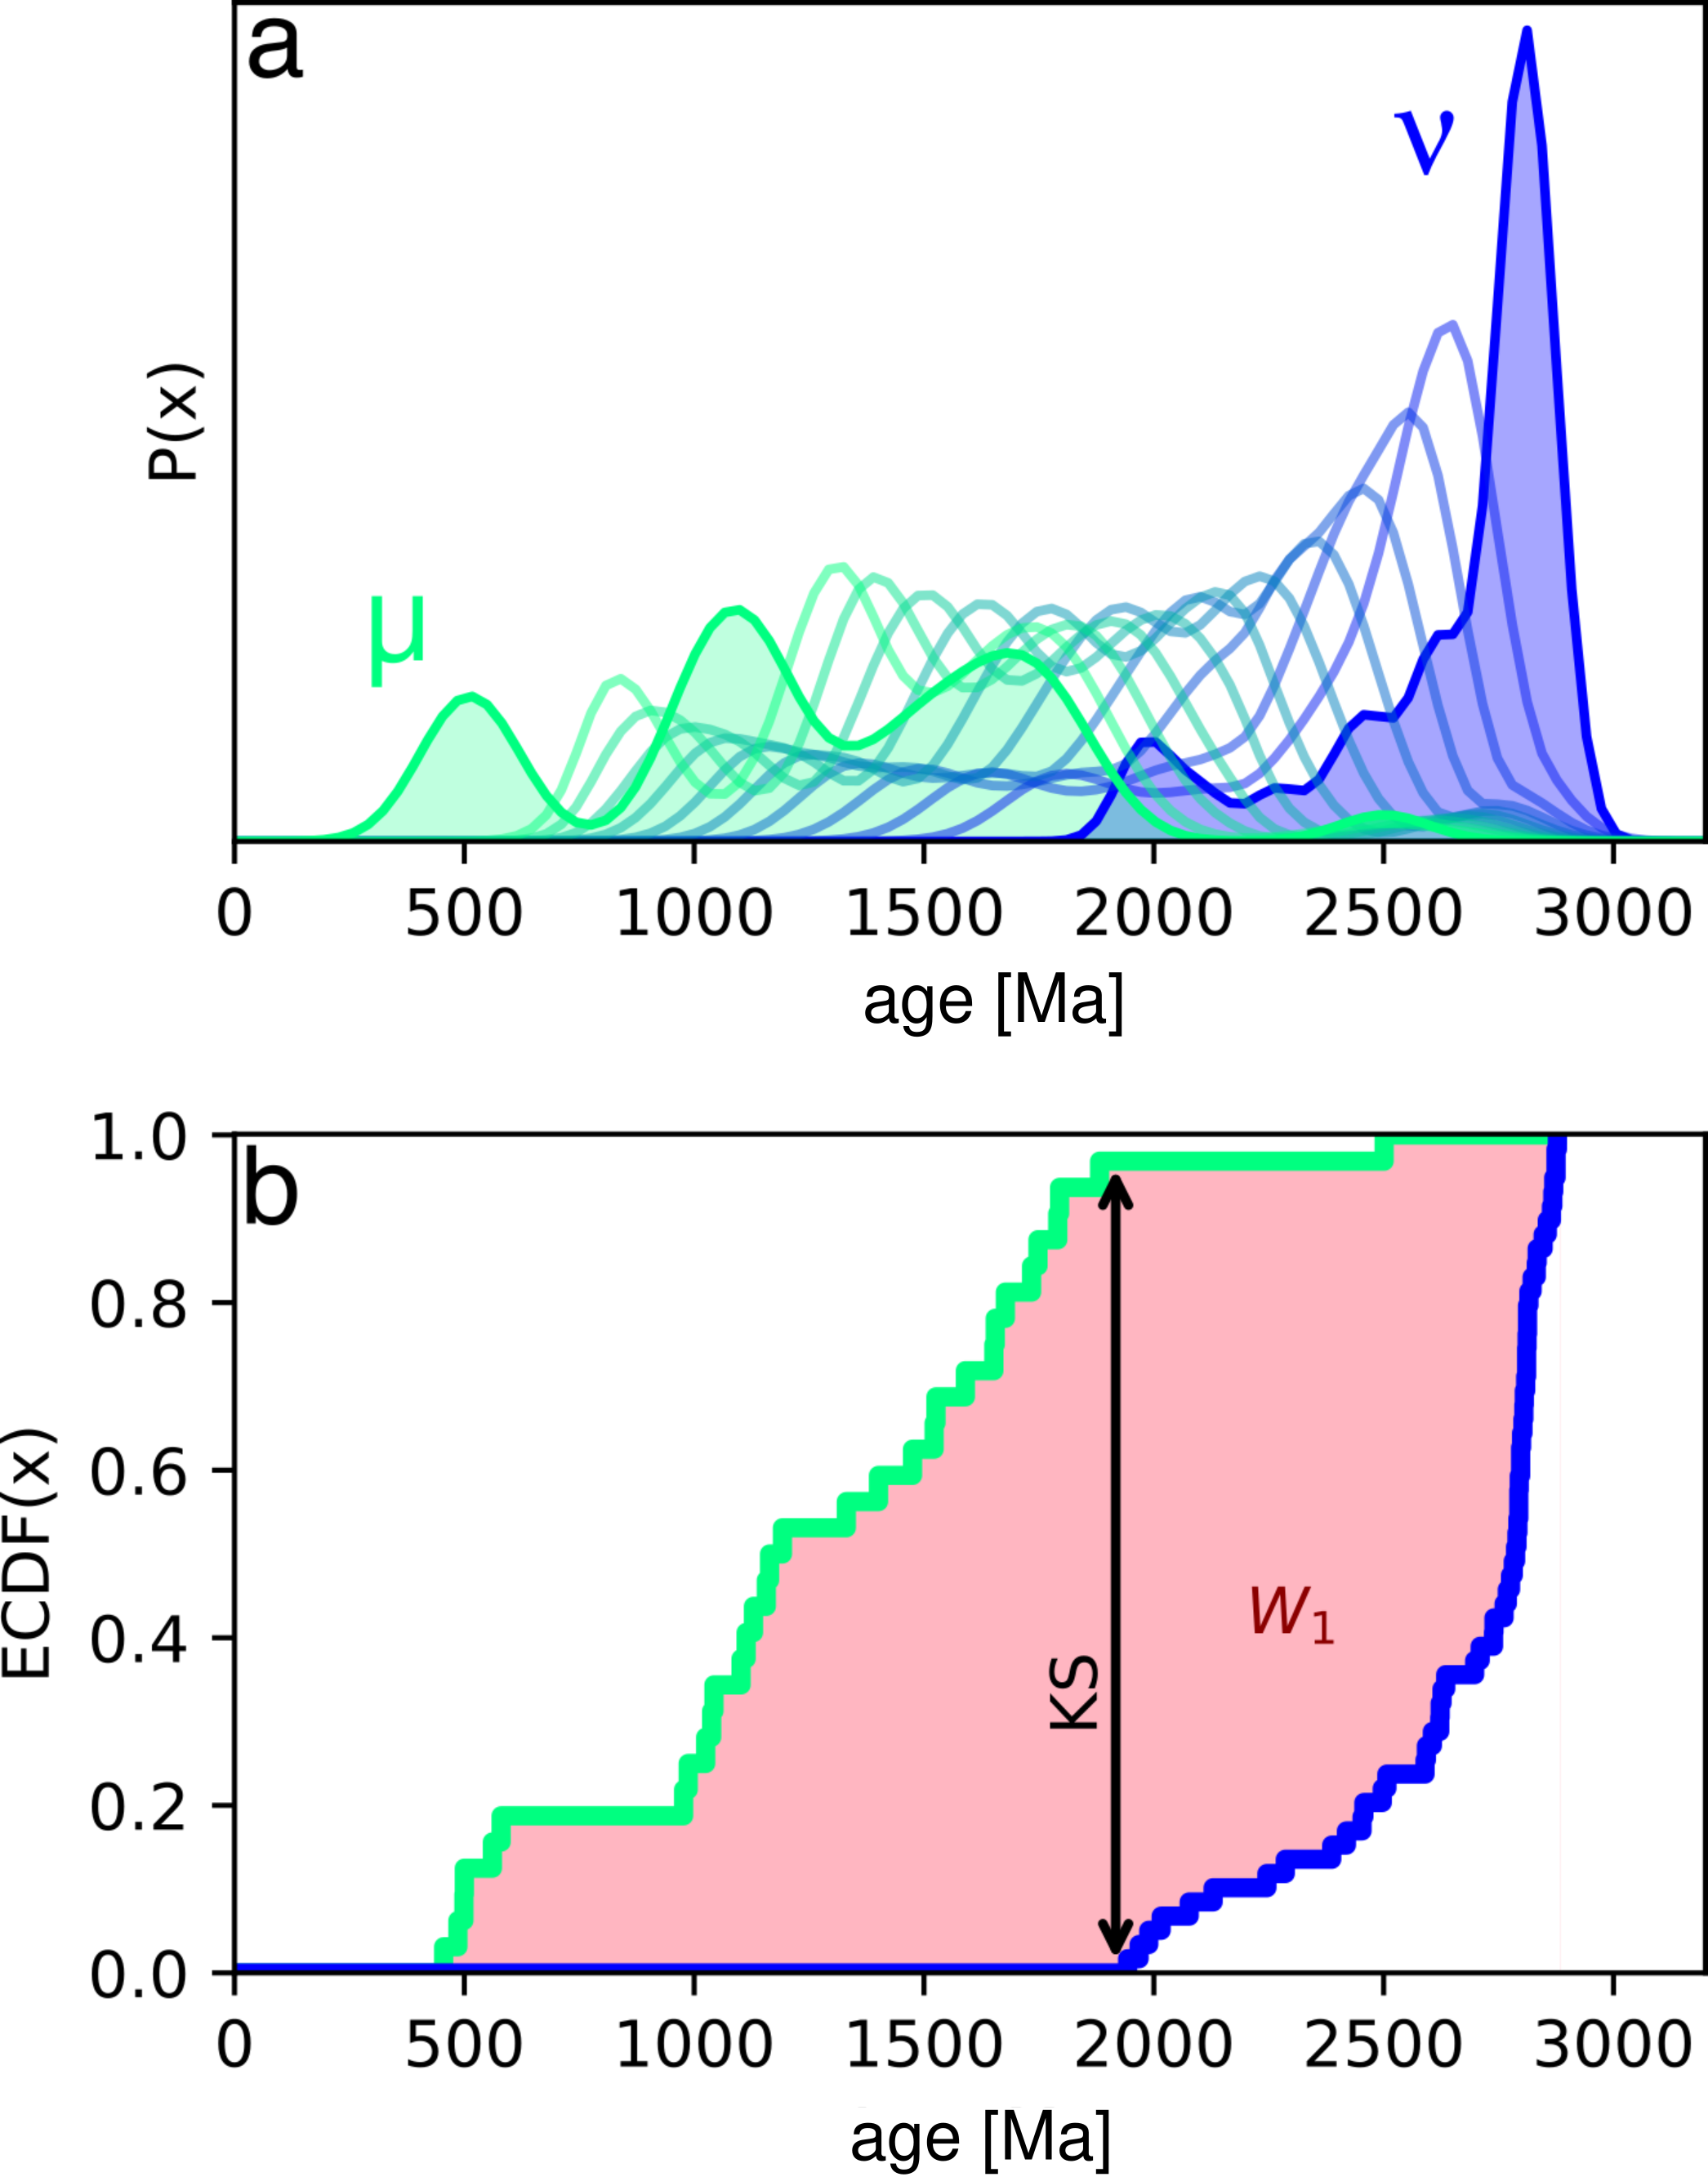
\includegraphics[width=\textwidth]{fig01.pdf}
  \end{minipage}\hfill
  \begin{minipage}[c]{0.45\textwidth}
    \caption{SIMS U--Pb calibration curve. White circles mark the
      isotopic measurements of the reference material, black circles
      those of two aliquots of the same sample. The uncertainty of the
      linear fit is shown as a 95\% confidence interval (grey area).
      This uncertainty can be propagated into the Pb/U-composition of
      the sample. It is a systematic uncertainty in the sense that it
      affects both aliquots. But it does not do so to the same
      degree. The calibration uncertainty of aliquot~2 is greater than
      that of aliquot~1, due to its horizontal offset relative to the
      calibration data.}
    \label{fig:syserr}
  \end{minipage}
\end{figure}

\section{U--Pb geochronology as a compositional data problem}
\label{sec:compositional}

Section~\ref{sec:accuracy} pointed out that the U--Pb age equation
(Equation~\ref{eq:tUPb}) does not depend on the absolute amounts of
\textsuperscript{204}Pb, \textsuperscript{206}Pb and
\textsuperscript{238}U, but only on their relative abundances.  Thus
we could normalise the \textsuperscript{204}Pb,
\textsuperscript{206}Pb and \textsuperscript{238}U measurements of
Table~\ref{tab:UPb} to unity and plot them on a ternary diagram.  The
same is true for other geochronometers such as U--Th--He and
\textsuperscript{40}Ar/\textsuperscript{39}Ar
\citep{vermeesch2010a,vermeesch2015b}. In mathematics, the ternary
sample space is known as a two-dimensional \textit{simplex}. Data that
live within this type of space are called \emph{compositional}
data.\medskip

Ternary systems are common in igneous petrology (e.g., the A--F--M
diagram) and sedimentary petrography (e.g., the Q--F--L
diagram). Geologists have long been aware of the problems associated
with averages, confidence regions, and linear regression in these
closed dataspaces \citep{chayes1949, chayes1960}.  But a general
solution to this conundrum was not found until the 1980s, when the
Scottish statistician John Aitchison published a landmark paper and
book on the subject \citep{aitchison1982, aitchison1986}.\medskip

In this work, Aitchison proved that all the problems associated with
the statistical analysis of compositional data can be solved by
mapping those data from the simplex to a Euclidean space by means of
an additive logratio (ALR) transformation.  For example, given the
ternary system $\{x,y,z\}$, we can define two new variables $\{u,v\}$
so that:
\begin{equation}
  u = \ln(x/z) \mbox{~and~} v = \ln(y/z)
  \label{eq:xyz2uv}
\end{equation}

In this space, Aitchison showed, one can safely calculate averages and
confidence limits.  Once the statistical analysis of the transformed
data has been completed, the results can then be mapped back to the
simplex by means of an inverse logratio transformation:
\begin{equation}
  x = \frac{e^u}{1+e^u+e^v} \mbox{,~}
  y = \frac{e^v}{1+e^u+e^v}
  \mbox{~and~} z = \frac{1}{1+e^u+e^v}
  \label{eq:uv2xyz}
\end{equation}

For example, the \textsuperscript{204,6}Pb--\textsuperscript{238}U
system of Table~\ref{tab:UPb} can be mapped from the ternary diagram
to a bivariate
$\ln({}^{204}$Pb/${}^{238}$U)--$\ln({}^{206}$U/${}^{238}$U)-space:\medskip

\begin{tabular}{r|cccccccccc}
  $u = \ln\!\left[\frac{{}^{206}\mbox{Pb}}{{}^{238}\mbox{U}}\right]$ &
  -2.46 & -2.82 & -2.30 & -1.10 & -2.32 & -1.47 & -2.09 & -0.82 & -2.01 & -2.87\\
  $v = \ln\!\left[\frac{{}^{204}\mbox{Pb}}{{}^{238}\mbox{U}}\right]$ &
  -7.23 & -6.59 & -7.17 & -9.48 & -7.60 & -7.79 & -8.05 & -8.94 & -8.38 & -6.25
\end{tabular}\medskip

Alternatively, we could also use \textsuperscript{206}Pb as the
denominator isotope:\medskip

\begin{tabular}{r|cccccccccc}
  $u = \ln\!\left[\frac{{}^{238}\mbox{U}}{{}^{206}\mbox{Pb}}\right]$ &
  2.46 & 2.82 & 2.30 & 1.10 & 2.32 & 1.47 & 2.09 & 0.82 & 2.01 & 2.87\\
  $v = \ln\!\left[\frac{{}^{204}\mbox{Pb}}{{}^{206}\mbox{Pb}}\right]$ &
  -4.77 & -3.77 & -4.88 & -8.38 & -5.28 & -6.31 & -5.96 & -8.12 & -6.37 & -3.39
\end{tabular}\medskip

Calculating the average of the transformed data and mapping the
results back to the simplex using the inverse logratio transformation
yields the \emph{geometric} mean of the ratios:
\[
\left(\overline{{}^{238}\mbox{U}/{}^{206}\mbox{Pb}}\right)_{\!g} =
7.58 = \frac{1}{0.13} = 
  \frac{1}{\left(\overline{{}^{206}\mbox{Pb}/{}^{238}\mbox{U}}\right)_{\!g}}  
\]

\noindent which is an altogether more satisfying result than in
Section~\ref{sec:accuracy}. Moving on to the 95\% confidence intervals
of the \textsuperscript{206}Pb/\textsuperscript{204}Pb-ratios, we
first determine the conventional confidence limits for the logratios:

\begin{center}
\begin{tabular}{ccccc}
  $u$ & $\bar{u}$ & $s_u$ &
  $\bar{u}+\frac{s_u}{\sqrt{10}}t^{2.5}_{9}$ &
  $\bar{u}+\frac{s_u}{\sqrt{10}}t^{97.5}_{9}$ \\ \hline
  log($^{206}$Pb/$^{204}$Pb) & 5.72 & 1.66 & 4.53 & 6.91 \\
\end{tabular}
\end{center}

After the inverse-logratio transformation, these values produce an
asymmetric 95\% confidence interval for the geometric mean
\textsuperscript{206}Pb/\textsuperscript{204}Pb-ratio of
$305^{+695}_{-212}$. This interval contains only strictly positive
values, solving the problem of Section~\ref{sec:precision}. The ALR
transformation of Equation~\ref{eq:xyz2uv} can easily be generalised
to more than three components. For example, if \textsuperscript{207}Pb
is added to the mix, then the four-component
\textsuperscript{$204|6|7$}Pb--\textsuperscript{238}U-system can be
mapped to the three component $\ln({}^{204|6|7}$Pb/${}^{238}$U)-space
(Figure~\ref{fig:ternaryUPb}).\medskip

The compositional nature of isotopic data embeds a covariant structure
into the very DNA of geochronology: in a $K$-component system,
increasing the absolute amount of one of the components automatically
lowers the relative amount of the remaining ($K$-1) components
\citep{chayes1960}. To deal with this phenomenon, it is customary in
compositional data analysis to process data in matrix form, using the
full covariance matrix. For example, four components yield three
logratios, which require a ${3}\times{3}$ covariance matrix to
describe the uncertainties and uncertainty correlations.\medskip

This approach is now widely used in sedimentary geology, geochemistry
and ecology \citep[e.g.,][]{weltje2002, vermeesch2006b,
  pawlowsky2011}, and has recently been adopted for geochronological
applications as well \citep{vermeesch2010a, vermeesch2015b,
  mclean2016}. The logratio covariance matrix approach is also
uniquely suited to capture the systematic uncertainties (i.e. the
inter-spot error correlations) that are produced by the SIMS U--Pb
calibration procedure (Section~\ref{sec:syserr}). In that case, the
covariance matrix must be expanded to accommodate multiple spots
\citep[e.g.,][]{vermeesch2015b}. For example, the covariance structure
of three spots in a four component system can be captured in a
${9}\times{9}$ matrix.\medskip

In conclusion, the logratio transformation solves the statistical woes
described in Sections~\ref{sec:accuracy}, \ref{sec:precision} and
\ref{sec:syserr} of this paper.  However there are two additional
problems that require further remediation.

\begin{figure}[!ht]
  \centering
  \includegraphics[width=.85\textwidth]{fig02b.pdf}
  \caption{The U--Pb age equation (a) projected onto the
    four-component simplex, and (b) mapped to a three-dimensional
    Euclidean logratio space. \textsuperscript{235}U is omitted from
    the diagrams because it exists in a constant ratio to
    \textsuperscript{238}U
    \citep[\textsuperscript{238}U/\textsuperscript{235}U=137.818,][]{hiess2012}. The
    boundaries between the coloured regions mark mixing lines between
    radiogenic and inherited end-member compositions, assuming common
    Pb ratios of
    [\textsuperscript{207}Pb/\textsuperscript{204}Pb]\textsubscript{c}
    = 10 and
    [\textsuperscript{206}Pb/\textsuperscript{204}Pb]\textsubscript{c}=9. The
    mixing lines define isochron surfaces that are linear in the
    simplex and curved in logratio space. Rotating the logratio plot
    $90^\circ$ clockwise produces a logarithmic version of the
    familiar Wetherill concordia diagram. Concordant
    \textsuperscript{206}Pb/\textsuperscript{238}U and
    \textsuperscript{207}Pb/\textsuperscript{235}U compositions are
    marked by a thick black line from 0 to 4Ga, and by a dotted line
    beyond 4Ga. This paper makes the case that U-Pb data processing is
    best done in logratio space, because this `liberates' the data
    from the geometric constraints of the simplex, producing symmetric
    uncertainty distributions and more accurate results.}
  \label{fig:ternaryUPb}
\end{figure}

\section{Background correction}
\label{sec:blanks}

Many mathematical operations are easier in logarithmic space than in
linear space: multiplication becomes addition, division becomes
subtraction, and exponentiation becomes multiplication. These
mathematical operations are very common in mass spectrometer data
processing chains \citep{vermeesch2015b}. However there are
exceptions. For example, background correction does not involve the
multiplication but subtraction of two signals. For low intensity ion
beams such as \textsuperscript{204}Pb it is possible, by chance, that
the background exceeds the signal.  This results in negative values of
which one cannot take the logarithm.\medskip

The subtraction problem can be solved by using a different logarithmic
change of variables:
\begin{equation}
  \beta^y_x \equiv \ln\!\left(\frac{y - b}{x - b}\right)
\end{equation}

\noindent where $x$ and $y$ are the signals and $b$ is the
background. The infinite space of $\beta^y_x$ covers all possible
values of $x$, $y$ and $b$ for which $x > b$ and $y > b$.  Thus,
background correction should be done in $\beta$-space, given an
appropriate error model as described in
Section~\ref{sec:counts}.\medskip

One caveat to this background correction method is that it does not
account for isobaric interferences, which may result in `overcounted'
signals. The high mass resolution of SIMS instruments removes most but
not all isobaric interferences. For example, spurious HfSi, REE
dioxide, or long-chain hydrocarbon ions can interfere with
\textsuperscript{204}Pb, which is generally the rarest isotopic
species detected. If unaccounted for, these interferences lead to the
proportion of non-radiogenic Pb being overestimated (and the
proportion of radiogenic Pb underestimated), resulting in excessive
common Pb corrections, and underestimated dates.  The accuracy of the
background measurements can be monitored via the use of isotopically
homogeneous reference materials \citep{black2005}. A correction can
then be applied by choosing the `session blank' that brings the
common-Pb corrected
\textsuperscript{207}Pb/\textsuperscript{206}Pb-ratios in alignment
with the reference values.\medskip

Another issue arises when SIMS signals are registered by Secondary
Electron Multiplier (SEM) detectors. These record ion beams as
discrete counts, i.e. as integers, which are incompatible with the
logratio transformation. For example, it is not uncommon for SEM
detectors to register zero counts for low intensity ion beams such as
\textsuperscript{204}Pb.  These zero counts blow up the logratio
transformation, because $\ln(0)=-\infty$.\medskip

This and other issues are diagnostic of a fundamental difference
between compositional data and counting data that has been previously
recognised and solved in fission track dating \citep{galbraith2005}
and in sedimentary petrography \citep{vermeesch2018d}.  The same
solutions can be applied to mass spectrometric count data in general,
and to U--Pb geochronology in particular (Section~\ref{sec:counts}).

\section{Dealing with count data}
\label{sec:counts}

Standard data reduction procedures for geochronology assume normally
distributed residuals. In compositional data analysis, these are
replaced by logistic normal distributions. However, neither the normal
nor the logistic normal distribution are perfectly suited to dealing
with discrete count data. The multinomial distribution is a simple
alternative that seems more appropriate for the task at hand. Before
we proceed, let us define the following variables:

\begin{itemize}
\item $\phi_{x}$ and $\phi_{b}$: the normalised true ion beam
  intensities (in counts per second) of mass $x$ (from a set of
  monitored masses $\mathbb{x}$) and the normalised background signal,
  respectively, so that
  \begin{equation}
    \phi_b + \sum_{{x}\in\mathbb{x}}\phi_{x} =1
  \end{equation}
\item $d_x$, $d_b$: the dwell times of mass $x$ and the background $b$
\item $\theta_{x}$ and $\theta_b$: the normalised expected beam
  \emph{counts} of the ions and the background, so that
\begin{equation}
  \theta_{x} = \frac{\phi_{x}d_{x}}
        {\phi_bd_b + \sum_{y\in\mathbb{x}}\phi_{y}d_y}
        \label{eq:thetax}
\end{equation}
\noindent and
\begin{equation}
  \theta_b + \sum_{x\in\mathbb{x}}\theta_{x} =1
\end{equation}
\end{itemize}

Then the probability of observing $n_4$ counts at mass 204, $n_6$
counts at mass 206 and $n_b$ counts of background is given by
\begin{equation}
  p(n_4,n_6,n_b|\theta_4,\theta_6,\theta_b) = 
  \frac{(n_4\!\!+\!n_6\!+\!n_b)!}{n_4!n_6!n_b!}
  \theta_4^{n_4}\theta_6^{n_6}\theta_b^{n_b}
  \label{eq:p46b}
\end{equation}

Whereas the observations $n_4$, $n_6$ and $n_b$ are integers, the
parameters $\theta_4$, $\theta_6$ and $\theta_b$ are decimal numbers
that are constrained to a constant sum. In other words, they belong to
the simplex. Thus, we can map the three multinomial parameters to two
logratio parameters, thereby establishing a natural link between
counting data and compositional data. For example:
\begin{align}
  \beta^{4}_{6} & \equiv
  \ln\!\left(\frac{\phi_4-\phi_b}{\phi_6-\phi_b}\right) = 
  \ln\!\left(\frac{\theta_4/d_4-\theta_b/d_b}{\theta_6/d_6-\theta_b/d_b}\right) \mbox{~and~} \\  
  \beta^{b}_{6} & \equiv
  \ln\!\left(\frac{\phi_b}{\phi_6-\phi_b}\right) = 
  \ln\!\left(\frac{\theta_b/d_b}{\theta_6/d_6-\theta_b/d_b}\right)
\end{align}

$\beta^{4}_{6}$ and $\beta^{b}_{6}$ can be estimated from $n_4$, $n_6$
and $n_b$ by maximising the likelihood defined by
Equation~\ref{eq:p46b}.\medskip

The normal and logistic normal distributions are controlled by two
sets of parameters: location parameters and shape parameters. In the
case of the normal distribution, the location parameter is the mean
and the shape parameter is the standard deviation (or covariance
matrix). In contrast, the multinomial distribution has only one set of
($\theta$) parameters.  The precision of multinomial counts is
governed by the number of observed counts ($\sigma[n] =
\sqrt{n}$). More sophisticated models are possible when the observed
dispersion of the data exceeds that which is expected from the
multinomial counting statistics
\citep[e.g.,][]{galbraith1993,vermeesch2018d}. However in this paper
we will assume that such \emph{overdispersion} is absent from the
reference materials, and from the single-spot analyses.

\section{Dead-time correction}
\label{sec:dead-time}

It takes a few tens of nanoseconds for a secondary electron multiplier
to record the arrival of an ion. During this `dead-time', the detector
is unable to register the arrival of additional ions. This phenomenon
can significantly bias isotope ratio estimates that include ion beams
of contrasting intensity. Fortunately, the dead-time effect can be
easily corrected.  It suffices that the dwell times are adjusted by
the cumulative amount of time that the detectors were incapacitated.
Let $d'_x$ be the `effective dwell time' of ion beam $x$:
\begin{equation}
  d'_x = d_x - n_x \delta_x
\end{equation}

\noindent where $\delta_x$ is the (non extended) dead-time of the detector
that measures $x$. Then the expected normalised beam counts can be
re-defined as:
\begin{equation}
  \theta'_{x} = \frac{\phi_{x}d'_{x}}
        {\phi_bd'_b + \sum_{y\in\mathbb{x}}\phi_{y}d'_y}
        \label{eq:thetax'}
\end{equation}

\noindent and the normalised beam intensities as
\begin{equation}
  \phi'_{x} = \frac{\theta_{x}/d'_{x}}
        {\theta_b/d'_b + \sum_{y\in\mathbb{x}}\theta'_{y}/d_y}
        \label{eq:phix'}
\end{equation}

The difference between this approach and existing SIMS data reduction
approaches is that conventional data reduction algorithms apply the
dead-time correction to the raw data, before calculating isotopic
data; whereas the new method applies the dead-time correction to
$\theta'_x$ and $\phi'_x$, which are unknown parameters that must be
estimated from the data.

\section{Within-spot drift correction}
\label{sec:drift}

Thus far we have assumed that all ions are measured synchronously,
which is the case in multicollector configurations. However in single
collector experiments, the measurements are made asynchronously. This
can cause biased results if the signals drift over time.  In SHRIMP
data processing, it is customary to correct this drift by normalising
to a secondary beam monitor (SBM) signal\footnote{SBM normalisation is
not a magic bullet. For example, whereas the \textsuperscript{206}Pb
signal of SHRIMP spot \texttt{M127.1.2} rises with time
(Figure~\ref{fig:timeresolved}b), its corresponding SBM signal
drops.}, followed by double interpolation of numerator and denominator
isotopes \citep{bodorkos2020, dodson1978}. A unified data reduction
algorithm for SHRIMP and Cameca instruments requires a different
approach, in which the time dependency of the signals is parameterised
using a log-linear model.  For Faraday detectors:
\begin{equation}
  n_x^i = \mbox{bkg} + \mathcal{N}(\exp[\alpha_x+\gamma_{X}\tau_x^i],\sigma^2)
  \label{eq:FARdrift}
\end{equation}

\noindent where $n_x^i$ is the ion beam intensity of the
$i$\textsuperscript{th} integration for mass $x$ of element $X$
evaluated at time $\tau_x^i$, $\sigma$ is the standard deviation of
the normally distributed data scatter around the best fit line, and
`bkg' is the background signal. This is usually a nominal value for
Cameca instruments and an actual set of measurements ($n_b^i$) for
SHRIMP data.  Note that the intercept parameters ($\alpha_x$) are
ionic mass-specific, whereas the slopes ($\gamma_X$) are
element-specific. See the Appendix for an example. For SEM detectors,
the scatter of the data around the log-linear fit is controlled by
Poisson shot noise:
\begin{equation}
  n_x^i \sim \mbox{bkg} +
  \mbox{Pois}\!\left(\exp[\alpha_x+\gamma_{X}\tau_x^i]d'_x\right)
  \label{eq:SEMdrift}
\end{equation}

The background-corrected signal ratio (evaluated at $\tau_x^i$) for
two ion beams $x$ and $y$ of different elements $X$ and $Y$ can then
be drift corrected as follows:
\begin{equation}
{}^{i}\!\beta^{y}_{x} \equiv
\ln\!\left(\frac{\phi^i_y-\phi^i_b}{\phi^i_x-\phi^i_b}\right) +
\gamma_Y\left(\tau_x^i-\tau_y^i\right)
  \label{eq:betadrift}
\end{equation}

\noindent where $\phi^i_x$ and $\phi^i_y$ are the dead time corrected
normalised beam intensities for the $i$\textsuperscript{th}
integration of masses $x$ and $y$, respectively, and $\phi^i_b$ is the
corresponding background value. See the Appendix for further details.

\section{Fractionation}
\label{sec:fractionation}

Mass spectrometer signals are recorded in Volt (for Faraday detectors)
or Hertz (or secondary electron multipliers). The age equation,
however, requires atomic ratios. In general, signal ratios do not
equal atomic ratios, because they are affected by two types of
fractionation:

\begin{enumerate}
\item{Mass-dependent fractionation:} The Pb-isotopes span a range of
  four mass units, with \textsuperscript{208}Pb being 2\% heavier than
  \textsuperscript{204}Pb. Both the production and detection
  efficiency of secondary ions vary with atomic mass, and significant
  errors can potentially occur if the resulting mass fractionation is
  uncorrected for. Mass fractionation can be quantified by comparing
  the measured signal ratios of a reference material with its known
  isotopic ratio. This is easy to do in a log-ratio context
  \citep{vermeesch2015b}.
\item{Elemental fractionation:} The fractionation between the
  Pb-isotopes is caused by (slight) differences in their physical
  properties, i.e. their mass. As briefly mentioned in
  Section~\ref{sec:syserr}, much stronger fractionation effects tend
  to occur between the isotopes and Pb and U, because they are not
  only physically, but also chemically different. These chemical
  differences affect the complex processes that occur when the primary
  ion beam interacts with the target material \citep{williams1998}.
\end{enumerate}

In the context of SIMS U--Pb geochronology, mass-dependent
fractionation is commonly ignored \citep[but not always,
  e.g.,][]{stern2009}, because the most important isochemical ratio is
that between \textsuperscript{206}Pb and \textsuperscript{207}Pb,
which lie within 0.5\% mass units of each other. This is unresolvable
given typical analytical uncertainties. The mass fractionation is
greater for \textsuperscript{204}Pb, but so it its analytical
uncertainty.  Therefore, the atomic
\textsuperscript{204}Pb/\textsuperscript{206}Pb,
\textsuperscript{207}Pb/\textsuperscript{206}Pb and
\textsuperscript{208}Pb/\textsuperscript{206}Pb ratios can be directly
estimated from the (drift corrected)
\textsuperscript{204}Pb/\textsuperscript{206}Pb,
\textsuperscript{207}Pb/\textsuperscript{206}Pb and
\textsuperscript{208}Pb/\textsuperscript{206}Pb signal ratios.  This
is not the case for the \textsuperscript{206}Pb/\textsuperscript{238}U
and \textsuperscript{208}Pb/\textsuperscript{232}Th-ratios, which are
affected by strong elemental fractionation effects. This fractionation
expresses itself in two ways:

\begin{enumerate}

\item{Within-spot fractionation}

Over the course of a SIMS spot analysis, the Pb/U and Pb/Th ratio
changes as a function of time. This elemental fractionation can be
modelled using a log-linear model that is similar to that used for the
within-spot drift correction:
\begin{equation}
  {}^{i}\!\beta^{y}_{x} = {}^{0}\!\beta^{y}_{x} + \gamma^{Y}_{X} \tau^i_x
  \label{eq:withinspotfractionation}
\end{equation}

\noindent where ${}^{0}\!\beta^{y}_{x}$ is the inferred logratio of
the background-corrected signals at `time zero', which can be found
using the method of maximum likelihood (see Appendix).  Note that
$\gamma_X^Y=0$ if $X=Y$ and, if the sensitivity drift of the data is
smooth and closely follows the trends defined by
Equations~\ref{eq:FARdrift} and \ref{eq:SEMdrift}, then
${}^{0}\beta_x^y \approx \alpha_y - \alpha_x$ and $\gamma^{Y}_{X}
\approx \gamma_Y - \gamma_X$.\medskip

Using Equation~\ref{eq:withinspotfractionation}, the isotopic logratios
can be interpolated (or extrapolated) to any point in time ($\tau$):
\begin{equation}
  {}^{\tau}\!\beta^{y}_{x} = {}^{0}\!\beta^{y}_{x} + \gamma^{Y}_{X} \tau
  \label{eq:betatau}
\end{equation}

The most precise values of ${}^{\tau}\!\beta^{y}_{x}$ are obtained
when $\tau$ is chosen in the middle of the analytical sequence.  These
values can be used for subsequent calculations.  Alternatively, we can
also use the time-zero intercepts ${}^{0}\!\beta^{y}_{x}$.

\item{Between-spot fractionation}

The Pb/U and Pb/Th signal ratios may vary between adjacent spots on
the same isotopically homogenous reference material. This
fractionation obeys the power law relationship given by
Equation~\ref{eq:Y=A+BX}.  Expressing this formula in terms of
corrected signal ratios:
\begin{equation}
  \ln\!\left[\frac{(\phi'_{6} - \phi'_b) - (\phi'_{4} -
      \phi'_b)(6/4)_c}{\phi'_{u} - \phi'_b}\right] = A + B
  \ln\!\left[\frac{\phi'_{o} - \phi'_b}{\phi'_{u} -
      \phi'_b}\right]
  \label{eq:UOUcalibration}
\end{equation}

\noindent where $(6/4)_c$ stands for the
\textsuperscript{206}Pb/\textsuperscript{204}Pb-ratio of the common Pb
(see the footnote of Section~\ref{sec:syserr}). Recasting
Equation~\ref{eq:UOUcalibration} in terms of the interpolated logratio
estimates:
\begin{equation}
  \ln\!\left[\exp({}^{\tau}\!\beta^6_u) -
    \exp({}^{\tau}\!\beta^4_u)(6/4)_c \right] = A + B ~ {}^{\tau}\!\beta^o_u
  \label{eq:calibration}
\end{equation}

\noindent where `$o$' stands for the uranium oxide
(\textsuperscript{238}U\textsuperscript{16}O$^{+}_{2}$ or
\textsuperscript{238}U\textsuperscript{16}O$^+$) and `$u$' stands for
\textsuperscript{238}U$^+$.

\end{enumerate}

\section{U--Pb age calculation}
\label{sec:calibrate}

Having applied Equation~\ref{eq:calibration} to a reference material
with known atomic \textsuperscript{206}Pb/\textsuperscript{238}U-ratio
$\left[{}^{206}\mbox{Pb}/{}^{238}\mbox{U}\right]^{\!r}_{\!a}$, the
atomic \textsuperscript{206}Pb/\textsuperscript{238}U-ratio of the
sample is given by
\begin{equation}
  \ln\!\left[\frac{{}^{206}\mbox{Pb}}{{}^{238}\mbox{U}}\right]^{\!s}_{\!a} =
  \ln\!\left[\frac{{}^{206}\mbox{Pb}}{{}^{238}\mbox{U}}\right]^{\!r}_{\!a} +
  {}^{\tau}\!\beta^6_u(sm) - A - B ~ {}^{\tau}\!\beta^o_u(sm)
  \label{eq:calibrate}
\end{equation}

\noindent where ${}^{\tau}\!\beta^6_u(sm)$ and
${}^{\tau}\!\beta^o_u(sm)$ are the interpolated logratio estimates of
the sample.  The \textsuperscript{206}Pb/\textsuperscript{238}U-age is
then obtained by plugging
$\left[{}^{206}\mbox{Pb}/{}^{238}\mbox{U}\right]^{\!s}_{\!a}$ into the age
equation. Uncertainties are obtained by standard error propagation
(see Appendix).

\section{Examples}\label{sec:examples}

The following paragraphs will illustrate the SIMS U--Pb data reduction
process using two datasets:

\begin{enumerate}
\item Dataset~1 was acquired by Dr. Yang Li at IGG-CAS Beijing, using
  a Cameca 1280HR instrument with five SEMs and two Faraday detectors
  that was run in single collector mode, using an SEM for all
  mass-stations. The dataset uses Temora2 zircon
  \citep[416.8$\pm$1.1~Ma,][]{black2004} as a reference material and
  91500 zircon \citep[1062.4$\pm$0.2~Ma,][]{wiedenbeck1995} as a
  sample. Measurements consist of seven cycles through a set of 11
  mass-stations per single spot measurement, for
  \textsuperscript{90}Zr\textsubscript{2}O (0.48 second dwell time per
  cycle), \textsuperscript{92}Zr\textsubscript{2}O (0.08~s), mass
  200.5 (background, 4.00~s), \textsuperscript{94}Zr\textsubscript{2}O
  (0.32~s), \textsuperscript{204}Pb (4.96~s), \textsuperscript{206}Pb
  (2.96~s), \textsuperscript{207}Pb (6.00~s), \textsuperscript{208}Pb
  (2.00~s), \textsuperscript{238}U (2.96~s), ThO\textsubscript{2}
  (2.96~s), and UO\textsubscript{2} (2.96~s).

\item Dataset~2 was acquired by Dr. Simon Bodorkos at Geoscience
  Australia using a single collector SHRIMP-II instrument, employing
  an SEM for all mass-stations. This dataset also uses Temora2 as a
  reference material, and 91500 zircon and OG.1
  \citep[3440.7$\pm$3.2~Ma,][]{stern2009} and M127
  \citep[524.36$\pm$0.16~Ma,][]{nasdala2016} as samples. Measurements
  consist of six cycles through a set of 10 mass-stations per single
  spot measurement, for \textsuperscript{90}Zr\textsubscript{2}O (2.0
  second dwell time per cycle), \textsuperscript{204}Pb (20~s), mass
  204.04091 (background, 20~s), \textsuperscript{206}Pb (15~s),
  \textsuperscript{207}Pb (40~s), \textsuperscript{208}Pb (5~s),
  \textsuperscript{238}U (5~s), ThO (2~s), UO (2~s), and
  UO\textsubscript{2} (2~s).
\end{enumerate}

\begin{figure}[!ht]
  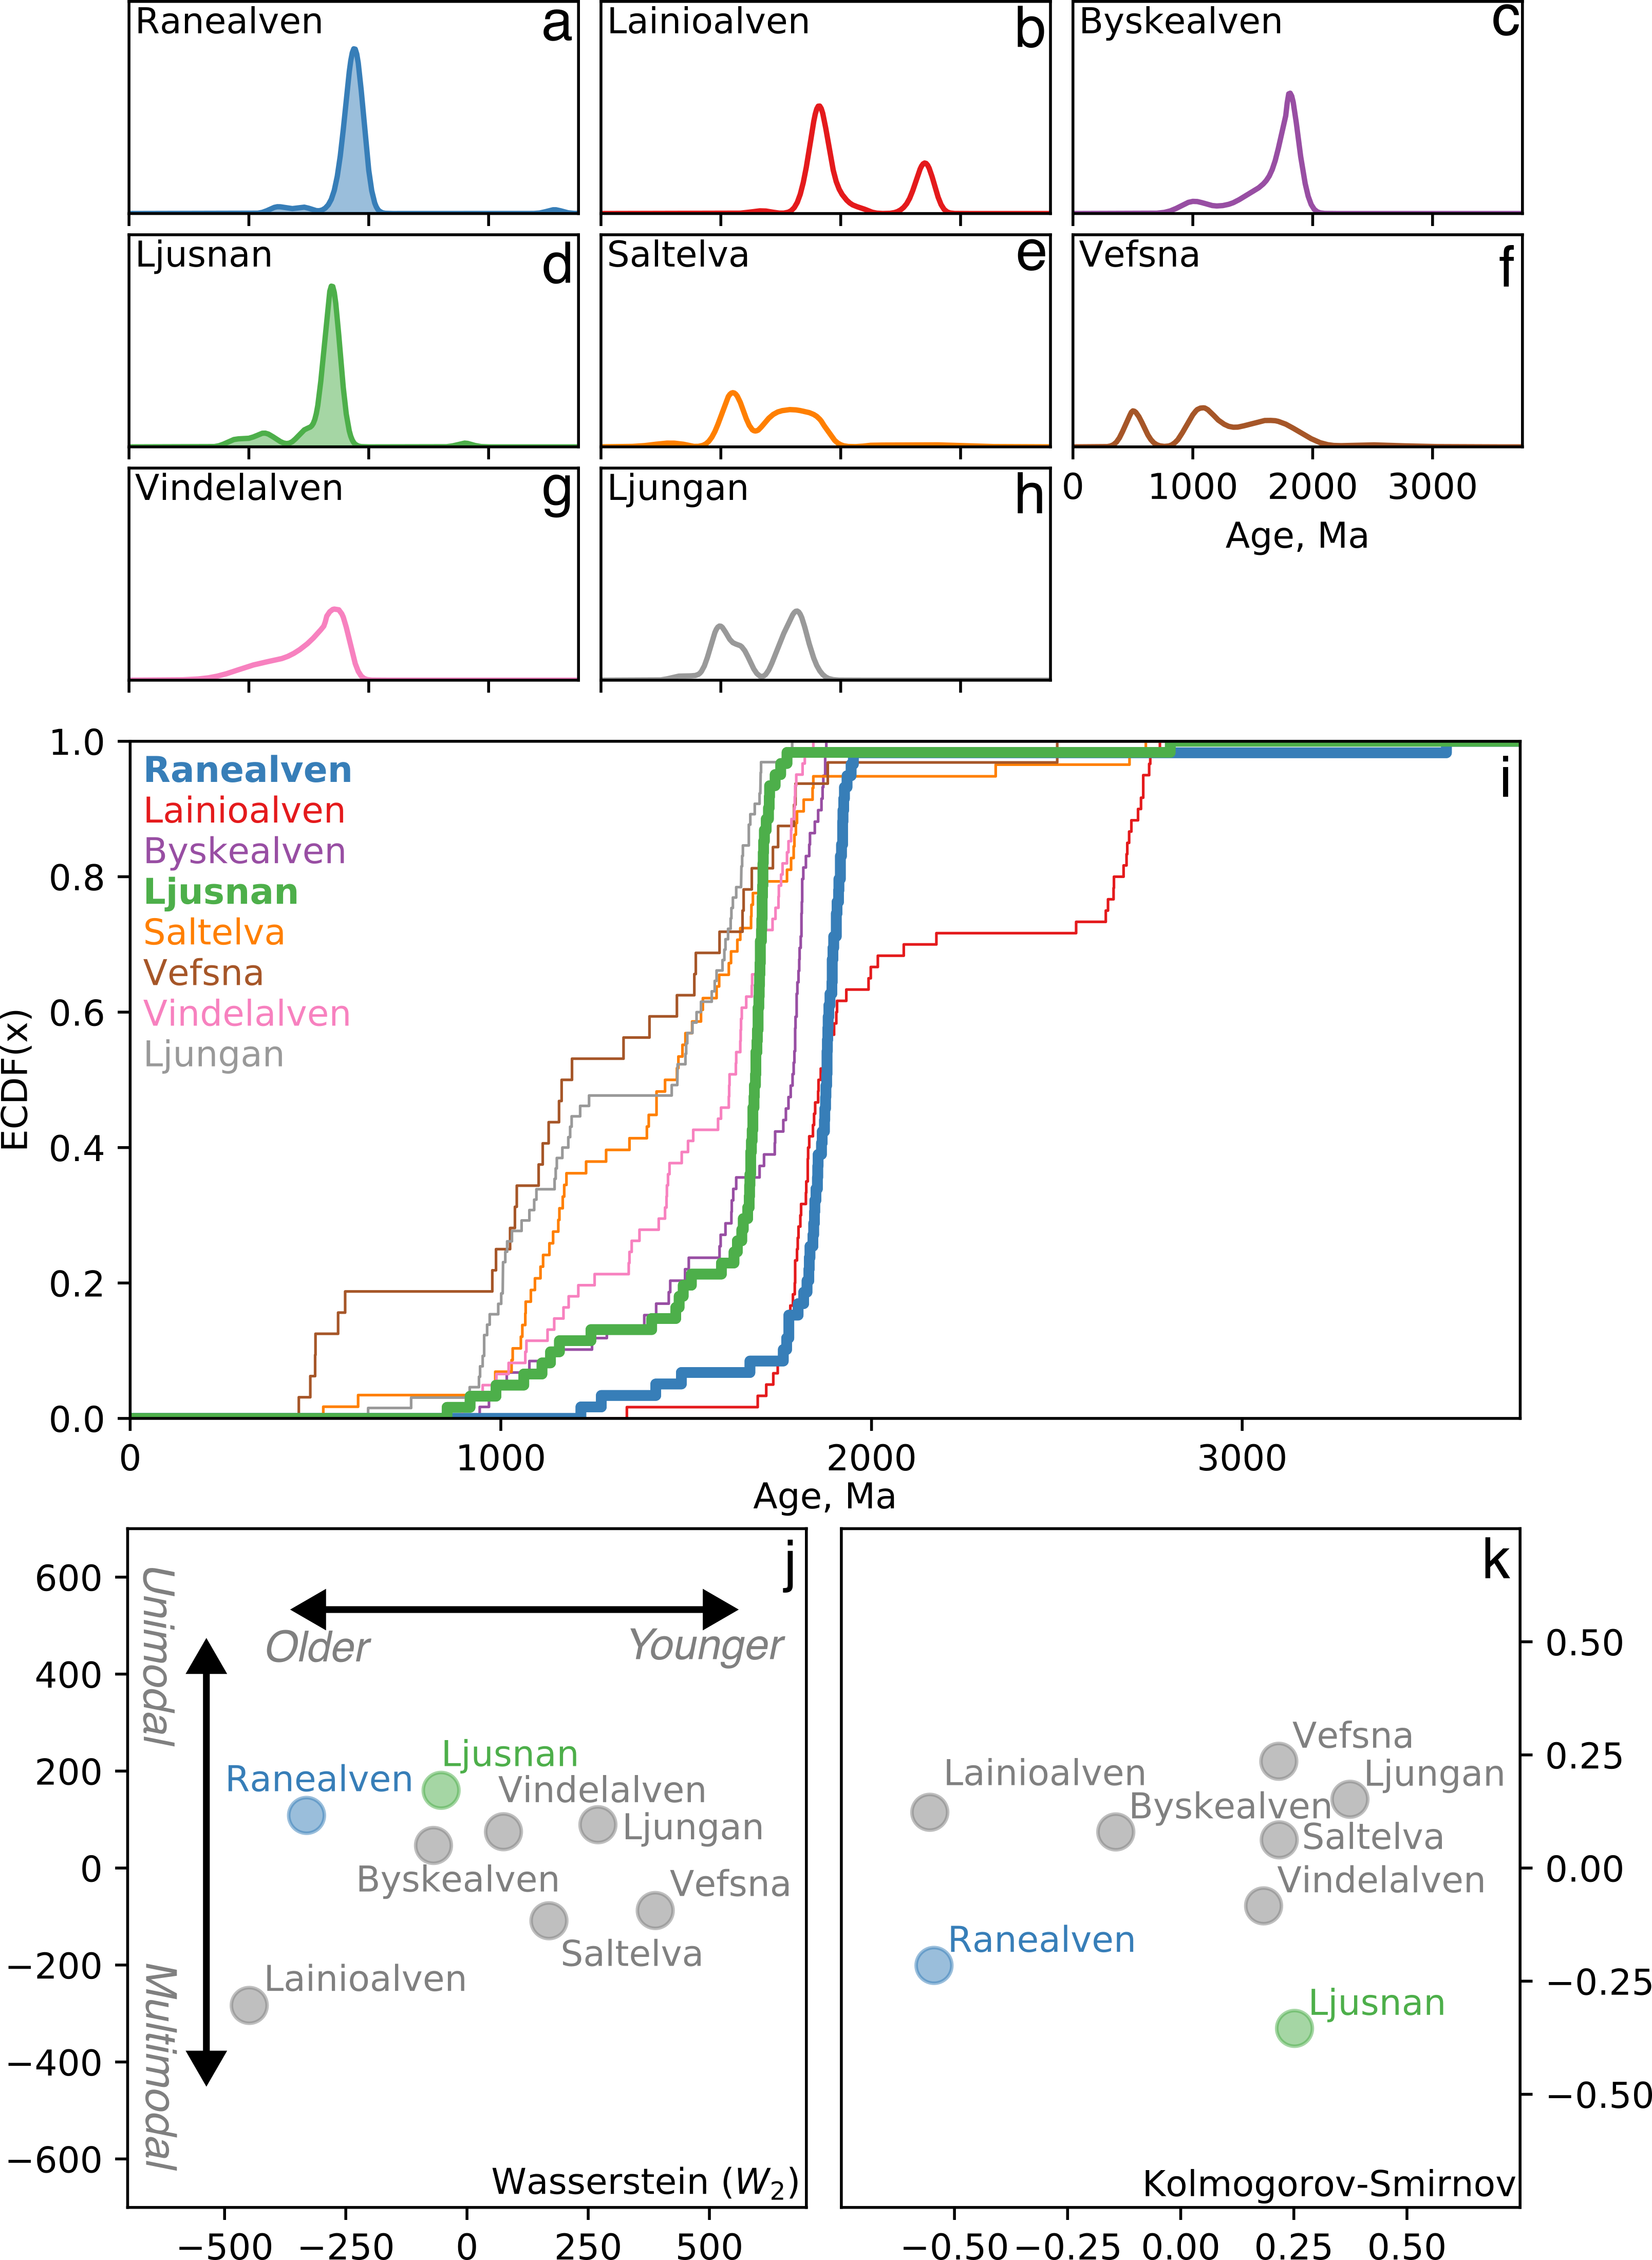
\includegraphics[width=\textwidth]{fig03.pdf}
  \caption{Time resolved signals (counts) of (a) Temora2 (spot
    \texttt{Tem@6}) analysed by a Cameca 1280HR instrument at IGG-CAS
    Beijing; (b) M127 zircon (spot \texttt{M127.1.2}) analysed by a
    SHRIMP-II instrument at Geoscience Australia.}
  \label{fig:timeresolved}
\end{figure}

Figure~\ref{fig:timeresolved} shows the time resolved SEM counts of
one representative spot measurement for each dataset. Side-by-side
comparison of these two datasets reveals some interesting similarities
and differences. All of the high intensity signals exhibit clear
transient behaviour, which is caused by changes in oxygen availability
that occur during primary ion bombardment \citep{magee2017}. The
transience of the individual SEM signals biases the isotopic
ratios. For example, there are 109 seconds between the
\textsuperscript{204}Pb and \textsuperscript{208}Pb measurements in
each SHRIMP cycle. During these 109 seconds, the
\textsuperscript{208}Pb signal drops on average by 2\%, resulting in
an equivalent bias of the
\textsuperscript{204}Pb/\textsuperscript{208}Pb ratio
(Section~\ref{sec:drift}). A similar drop per cycle is observed for
the Cameca data.\medskip

However, there is a key difference between the Cameca and SHRIMP
datasets. For the Cameca data, the U and Pb signals both drift in the
same direction, resulting in positive slopes for the example of
Figure~\ref{fig:timeresolved}. But for the SHRIMP data, the U- and
Pb-drifts act in opposite directions: the U-signal exhibits an
increase in sensitivity with time, whereas the Pb-signals decrease in
intensity with time.  This marked difference in behaviour between the
two instruments reflects a difference in their design, causing a
difference in the energy window of the secondary ions analysed
\citep{ireland2003}.\medskip

For Faraday detectors, the within-spot drift correction uses a
generalised linear model with a lognormal link function
(Equation~\ref{eq:FARdrift}).  For SEM data, it uses a Poisson link
function (Equation~\ref{eq:SEMdrift}).  In either case, the model
enforces strictly positive isotopic abundances. Isotopes of the same
element (such as \textsuperscript{$204|6|7|8$}Pb) have the same slope
parameter, but different intercepts. Isotopes of different elements
are free to have different slopes (Figure~\ref{fig:drift}).\medskip

\begin{figure}[!htbp]
  \centering
  \includegraphics[width=.7\textwidth]{fig04.pdf}
  \parbox{.7\textwidth}{
  \caption{Within-spot drift correction of the background-corrected
    SHRIMP data from Figure~\ref{fig:timeresolved}. Dotted lines are
    log-linear functions whose element-specific slopes ($\gamma_X$ in
    Equation~\ref{eq:SEMdrift}) are used for the drift correction but
    for no other purpose.  Solid lines mark the duration of each mass
    spectrometer cycle, with the black dots representing the starting
    point of each individual mass station within the cycles.  The
    solid lines are parallel to the dotted lines (in log space) and
    express how the isotope ratio fits can be translated to match the
    asynchronous mass spectrometer signals.  Vertical axes have units
    of counts per second.}
  \label{fig:drift}
  }
\end{figure}

Figure~\ref{fig:withinspotfractionation} applies another log-linear
function (Equation~\ref{eq:withinspotfractionation}) to model the
within-spot fractionation of Temora2 spot~11. This function models the
drift-corrected logratios as a linear function of analysis time. The
slopes of the log-linear functions are a function of the within-spot
fractionation between the numerator and denominator elements. Because
there is no fractionation between two isotopes of the same element,
the slope of the Pb/Pb ratios is zero.\medskip

The ability of logratio statistics to avoid negative ratios is
apparent from the first panel of
Figure~\ref{fig:withinspotfractionation}. Even though some of the
ratios of the background-corrected signals are zero or negative
(because the background exceeded the signal), the generalised linear
fit is strictly positive. The natural ability of compositional data
analysis to rule out negative ratios avoids many problems further down
the data processing chain.\medskip

The right hand side of Figure~\ref{fig:withinspotfractionation} maps
the four (log)ratios back to five equivalent raw signals (one for each
isotope). The last two panels of the figure show how the logratio
approach manages to effectively capture subtle fluctuations of the U
and UO signal intensities.\medskip

\begin{figure}[!htbp]
  \centering
  \includegraphics[width=\textwidth]{fig05.pdf}
  \parbox{\textwidth}{
  \caption{a) Background- and drift-corrected ratio fits to the SHRIMP
    data from Figure~\ref{fig:timeresolved}, obtained using the
    generalised linear model of
    Equation~\ref{eq:withinspotfractionation}. The slope parameter
    ($\gamma_X^Y$ in Equation~\ref{eq:withinspotfractionation}) is
    zero for isotopes of the same element and non-zero for isotopes of
    different elements. Vertical axes are unitless. b) The four
    (log)ratio fits can be converted back to five isotope signal fits
    using the inverse logratio transformation. Multiplying the
    normalised ion beam intensity fits with the total number of counts
    per sweep allows direct comparison with the raw measurements,
    which are shown as filled circles. Vertical axes have units of
    counts. Note that the measurements have Poisson uncertainties,
    which scale with the square root of the values.}
  \label{fig:withinspotfractionation}
  }
\end{figure}

The logratio intercepts obtained by
Equation~\ref{eq:withinspotfractionation} form a linear array of
calibration data
(Equation~\ref{eq:calibration}). Figure~\ref{fig:calibration}a fits a
straight line through these points using the linear regression
algorithm of \citet{york2004}. Alternatively, instead of fitting a
calibration line through the logratio intercepts ($\tau = 0$,
Figure~\ref{fig:calibration}a), it is also possible to interpolate or
extrapolate the logratio composition to any other point in time. For
example, the green ellipses in Figure~\ref{fig:calibration}b show the
inferred logratio compositions at 544 seconds (i.e., $\tau = 544$),
which represents the midpoint of the analyses. The slope of this
calibration line is notably different than that obtained by fitting a
line through the compositions at 0 seconds. This change in slope
reflects the different mechanisms that are responsible for elemental
fractionation within and between SIMS spots.\medskip

\begin{figure}[!htbp]
  \centering
  \includegraphics[width=\textwidth]{fig06.pdf}
  \parbox{\textwidth}{
  \caption{a) U--Pb calibration curve for the Temora2 SHRIMP data
    using the time-zero ($\tau = 0$) intercepts (green
    ellipses). Black and white dots mark the first and last cycles of
    each analysis, respectively. b) The logratio data and calibration
    fit for the same data, but evaluated at the midpoint ($\tau =
    544$), resulting in a more precise calibration. All uncertainties
    are shown at 95\% confidence.}
  \label{fig:calibration}
  }
\end{figure}

Figure~\ref{fig:91500} applies the Pb/U-calibration
(Equation~\ref{eq:calibrate}) to 91500 zircon, using the Temora2 data
for calibration. It shows only the purely random errors, i.e.,
ignoring the uncertainty of the calibration. Including the calibration
errors does not only inflate the uncertainties, but also causes
inter-spot error correlations (Figure~\ref{fig:syserr}). To
demonstrate this phenomenon, let us revisit the Cameca data and swap
the sample and reference materials around. Thus, we use 91500 for the
calibration curve, and Temora2 as a sample
(Figure~\ref{fig:Camecasyserr}). Table~\ref{tab:Camecasyserr} shows
the uncertainty budget of four selected aliquots from this
sample.\medskip

\begin{figure}[!htbp]
  \centering \includegraphics[width=\textwidth]{fig07.pdf}
  \caption{a) Calibration plot of the SHRIMP 91500 zircon data, using
    Temora2 as a reference material.  Dotted lines are parallel to the
    best fit line of Figure~\ref{fig:calibration}b.  b) The same data
    shown on a Tera-Wasserburg concordia diagram, which was obtained
    with \texttt{IsoplotR} and does not take into account systematic
    uncertainties associated with the calibration fit. All
    uncertainties are shown at 95\% confidence. The white ellipse
    marks the weighted mean composition, with MSWD and p-values
    representing the goodness of fit for equivalence, concordance, and
    equivalence + concordance.}
    \label{fig:91500}
\end{figure}

\begin{figure}[!htbp]
  \centering
  \includegraphics[width=0.6\textwidth]{fig08.pdf}
  \parbox{.6\textwidth}{
    \caption{Calibration curve of the Cameca data, using 91500 zircon
      as a reference material (top half of the plot), and Temora2
      zircon as a sample (bottom half). $a$--$d$ mark four Temora2
      aliquots whose uncertainty budget is explored in
      Table~\ref{tab:Camecasyserr}.  }
  \label{fig:Camecasyserr}
  }
\end{figure}

\begin{table}[!ht]
\centering
\begin{tabular}{rcccccc}
~ & ln[\textsuperscript{206}Pb/\textsuperscript{238}U] & int. unc. (\%) & tot. unc. (\%) & $r[*,b]$ & $r[*,c]$ & $r[*,d]$ \\ \hline
$a$ & -2.692 & 0.32 & 0.70 & 0.62 & 0.36 & -0.34 \cr
$b$ & -2.685 & 0.31 & 0.44 &      & 0.36 & -0.17 \cr
$c$ & -2.693 & 0.30 & 0.36 &      &      & 0.019 \cr
$d$ & -2.719 & 0.45 & 0.56 &      &      &      
\end{tabular}
\parbox{.6\textwidth}{
  \caption{Uncertainty budget of the four Temora2 zircon analyses
    highlighted in Figure~\ref{fig:Camecasyserr}. The first two data
    columns show the calibrated
    \textsuperscript{206}Pb/\textsuperscript{238}U logratios and their
    standard errors ignoring the uncertainty of the calibration fit
    (i.e., using internal uncertainties only). The third column shows
    the total error including the external uncertainty associated with
    the calibration fit.  The upper triangular matrix shown in the
    remaining three columns contain the (total) error correlations of
    the four aliquots.}
  \label{tab:Camecasyserr}
}
\end{table}

Propagating the calibration curve uncertainty increases the error
estimates (Table~\ref{tab:Camecasyserr}) by different amounts for
different spots. For aliquot $c$, which is located immediately below
the mean of the 91500 data, the calibration uncertainty only mildly
increases the standard error from 0.30\% to 0.36\%. However, for
aliquot $a$, which is horizontally offset from the mean of the
calibration data, the systematic calibration uncertainty more than
doubles the standard error from 0.32\% to 0.70\%. The calibration
error also causes the standard errors of the various aliquots to be
correlated with each other. For example, the total uncertainties of
aliquots $a$ and $b$ are positively correlated ($r[a,b]=0.62$) because
their UO\textsubscript{2}/U-ratios are both offset from the mean of
the calibration in the same direction.  In contrast, the uncertainties
of aliquots $a$ and $d$ are negatively correlated ($r[a,d]=-0.34$)
because they are offset in opposite directions from the mean of the
calibration data.\medskip

The inter-spot error correlations are important when calculating
weighted means \citep{vermeesch2015b} and isochrons. Taking into
account the full covariance structure of the data affects both the
accuracy and the precision of any derived age information.  For
example, the conventional weighted mean can be replaced with a matrix
expression that accounts for correlated uncertainties
\citep[Equation~92 of][]{vermeesch2015b}. Applying this modified
algorithm to the positively correlated aliquots $a$ and $b$ of
Table~\ref{tab:Camecasyserr} changes the weighted mean from $-2.6922$
to $-2.6854$ and increases the standard error of that mean from 0.37\%
to 0.44\%. Applying the same calculation to the negatively correlated
aliquots $a$ and $d$ changes their weighted mean from $-2.7083$ to
$-2.7076$ and reduces its uncertainty from 0.43\% to 0.35\%. To take
full advantage of the covariance matrix will require the development
of a new generation of high level data reduction software.  For
example, future versions of \texttt{IsoplotR} \citep{vermeesch2018c}
will be modified to handle these rich data structures.  A
comprehensive discussion of this topic falls outside the scope of this
paper.

\section{The \texttt{R} package \texttt{simplex}}\label{sec:simplex}

\texttt{simplex} is an \texttt{R} package for SIMS data processing
that implements the algorithm presented in this paper.  The program
can be run in three modes: online, offline, and from the command
line. The online version can be accessed at
\url{https://isoplotr.es.ucl.ac.uk/simplex/}. It contains three example
U--Pb datasets, including the two datasets used in this paper, plus a
Cameca monazite U--Th--Pb dataset.\medskip

\texttt{simplex} currently accepts raw data as Cameca \texttt{.asc}
and SHRIMP \texttt{.op} and \texttt{.pd} files. Support for SHRIMP
\texttt{.xml} files will be added later. The online version is a good
place to try the look and feel of the software. However, it is
probably not the most practical way to process lots of large data
files.  For a more responsive user experience, \texttt{simplex} can
also be run natively on any operating system (Windows, Mac OS or
Linux). To this end, the user needs to install \texttt{R} on their
system (see \url{https://r-project.org/} for details). Within
\texttt{R}, the \texttt{simplex} package can be installed from the
\texttt{GitHub} code-sharing platform using the \texttt{remotes}
package, by entering the following commands at the console:

\begin{verbatim}
install.packages("remotes")
remotes::install_github("pvermees/simplex")
\end{verbatim}

Once installed, \texttt{simplex}' graphical user interface (GUI) can
be started by entering the following command at the console:

\begin{verbatim}
simplex::simplex()
\end{verbatim}

A third and final way to use \texttt{simplex} is from the command
line.  This allows advanced users to create automation scripts and
extend the functionality of the package. \texttt{simplex} comes with
an extensive API (Application Programming Interface) of fully
documented user functions. An overview of all these functions can be
obtained by typing the following command at the console:

\begin{verbatim}
help(package="simplex")
\end{verbatim}

\section{Discussion}  %% \conclusions[modified heading if necessary]

This paper introduced a new algorithm for SIMS U--Pb geochronology, in
which raw mass spectrometer signals are processed using a combination
of logratio analysis and Poisson counting statistics. In contrast with
existing data reduction protocols, which handle each aliquot of an
analytical sequence separately, the new algorithm simultaneously
processes all of them in parallel. It thereby produces an internally
consistent set of isotopic ratios and their associated covariance
matrix. This covariance matrix is a rich source of information that
captures both random and systematic uncertainties, including
inter-spot error correlations that have hitherto been ignored in
geochronology.\medskip

The example data of Section~\ref{sec:examples} showed that these
inter-spot error correlation can be either positive or negative
\citep[see also][]{vermeesch2015b,mclean2016}. Ignoring them affects
both the accuracy and precision of high end data processing steps such
as isochron regression and concordia age calculation. Unfortunately,
existing postprocessing software such as \texttt{Isoplot}
\citep{ludwig2003} and \texttt{IsoplotR} \citep{vermeesch2018c} does
not yet handle inter-spot error correlations. Further work is needed
to extend these codes and take full advantage of the new
algorithm. \texttt{IsoplotR} was designed with such future upgrades in
mind: its input window contains a large number of spare columns that
will accommodate covariance matrices in a future update.  Once the
aforementioned high end data reduction calculations have been updated,
it will be possible to fully quantify the gain in precision and
accuracy of the new algorithm compared to the previous generation of
SIMS data reduction software.\medskip

The data reduction principles laid out in this paper are applicable
not only to U--Pb geochronology, but also to other SIMS applications
such as stable isotope analysis.  In fact, \texttt{simplex} already
handles such data for multicollector Cameca instruments.  It is worth
mentioning that the stable isotope functionality can also be used to
correct \textsuperscript{207}Pb/\textsuperscript{206}Pb ratio
measurements for mass-dependent isotope fractionation, as was briefly
discussed in Section~\ref{sec:fractionation}. Future updates of the
mass-dependent fractionation correction will also addresses the
overcounted background problem that was mentioned in
Section~\ref{sec:blanks}.\medskip

Besides U--Pb geochronology and stable isotopes, the new data
reduction paradigm can also be adapted to other chronometers and other
mass spectrometer designs, such as Thermal Ionisation Mass
Spectrometry \citep[TIMS,][]{connelly2021}, noble gas mass
spectrometry \citep{vermeesch2015b}, and LAICPMS \citep{mclean2016}.
\texttt{simplex} already includes a function to export data to
\texttt{IsoplotR}.  Adding similar functionality to other data
processing software will improve geochronologists' ability to
integrate multiple datasets whilst keeping track of systematic
uncertainties, including those associated with reference materials and
decay constants.

\section*{Appendix A}    %% Appendix A

This Section provides further algorithmic details for the new U--Pb
data processing workflow. It assumes that ions are recorded on SEM
detectors, which is by far the most common configuration. The case of
Faraday collectors is similar and, in fact, simpler.\medskip

Within-spot drift is modelled using a log-linear function
(Equation~\ref{eq:SEMdrift}) with a distinct intercept ($\alpha_x$)
for each ion channel ($x$), and shared slopes ($\gamma_X$) between
isotopes of the same element ($X$). To illustrate this concept,
consider the case of \textsuperscript{$204|6|7$}Pb (inclusion of
\textsuperscript{208}Pb is a trivial extension). Let $\hat{n}^i_x$ be
the time dependent parameter of the shot noise for ${}^{20x}$Pb, where
$x\in\{4,6,7\}$:
\begin{equation}
  \hat{n}^i_x = \mbox{bkg} + \exp(\alpha_x + \gamma_{Pb}t^i_x) d'_x
\end{equation}

\noindent then the log-likelihood function of the parameters given the
data is defined as:
\begin{equation}
  \mathcal{LL}_{d}\left(\alpha_{\{x\}},\gamma_{Pb}|n_{\mathbb{x}}^i\right) =
  \mbox{Const.} + \underset{x}{\sum} \sum\limits_{i=1}^{N}
  \left( n_x^i \ln\!\left[\hat{n}_x^i\right] - \hat{n}_x^i \right)
\end{equation}

\noindent where $N$ represents the number of cycles. The parameters
$\alpha_{\{x\}}=\{\alpha_4,\alpha_6,\alpha_7\}$ and $\gamma_{Pb}$ are
estimated by maximising $\mathcal{LL}_d$ with respect to them. Only
$\gamma_{Pb}$ is used in subsequent calculations.  The intercepts
$\alpha_{\{x\}}$ are discarded.\medskip

The next step of the data reduction extracts logratios from the raw
data using a log-linear model that is similar to the within-spot drift
correction (Equation~\ref{eq:withinspotfractionation}). Here, in
contrast with the drift correction, the intercepts are just as
important as the slopes. For isochemical ratios such as
\textsuperscript{207}Pb/\textsuperscript{206}Pb, the slope of the
drift-corrected logratios is zero and we only need to estimate the
intercept. For multichemical ratios such as
\textsuperscript{238}U/\textsuperscript{206}Pb, both the slope and the
intercept are non-zero. In order to keep track of covariances, it is
useful to process all the isotopes together, using a common
denominator. For example, using \textsuperscript{206}Pb (`6') as a
common denominator and \textsuperscript{204}Pb (`4'),
\textsuperscript{207}Pb (`7'), \textsuperscript{238}U (`$u$') and UO
(`$o$') as numerators:
\begin{equation}
  {}^{i}\!{\beta}^{x}_{6} =
  {}^{0}\!\beta_{6}^{x} + \gamma_{6}^{x} \tau_{6}^i +
  \gamma_{X} \left(\tau_{x}^i-\tau_{6}^i\right) + \ln[d_{6}'] - \ln[d_{x}']
\end{equation}

\noindent where `$X$' stands for Pb if $x\in\{4,6,7\}$, for U if
$x=u$, and for UO if $x=o$. Then the normalised ion counts are given
by:
\begin{equation}
  {\theta}^{i}_{y} = \exp\!\left[{}^{i}\!{\beta}_{6}^{y}\!\right]/D_i
  \mbox{~and~}
  {\theta}^{i}_{6} = 1/D_i
\end{equation}

\noindent for $y\in\{4,7,u,o\}$, with
\begin{equation}
  D_i = 1 + \underset{y}{\sum}
  \exp[{}^{i}\!{\beta}^y_6] + \frac{n^i_b}{\underset{z}{\sum}n^i_z}
\end{equation}

\noindent in which $z\in\{4,6,7,u,o,b\}$. Then the log-likelihood is
calculated as:
\begin{equation}
  \mathcal{LL}_l\left({}^{0}\!\beta_{6}^{\{x\}},\gamma_{6}^{\{x\}}|n_{\mathbb{x}}^i\right)
  = \mbox{Const.} + \sum\limits_{i=1}^{N}\underset{x}{\sum} n_x^i
  \ln[{\theta}_x^i]
\end{equation}

\noindent where $\gamma_6^4=\gamma_6^7=0$ because there is no
elemental fractionation between the Pb-isotopes. From the logratios
with common denominator, it is easy to derive any other logratio:
\begin{equation}
  {}^{\tau}\!\beta_{x}^{y} = {}^{\tau}\!\beta_{6}^{y} - {}^{\tau}\!\beta_{6}^{x}
\end{equation}

One of the main advantages of the new data reduction method is its
ability to keep track of the full covariance structure of the data,
including inter-spot error correlations. This ability is derived from
the fact that all parameters are derived by the method of maximum
likelihood, which stipulates that the approximate covariance matrix of
any set of estimated parameters can be obtained by inverting the
negative matrix of second derivatives (i.e., the Hessian matrix) of
the log-likelihood function with respect to said parameters:
\begin{equation}
  \Sigma \approx -\mathcal{H}^{-1}
\end{equation}

For example, to estimate the covariance matrix of the logratio slopes
and intercepts for a single spot analysis, the Hessian is a
${6}\times{6}$ matrix that includes the second derivatives of
$\mathcal{LL}_l$ with respect to $\beta_6^4$, $\beta_6^7$,
$\beta_6^u$, $\beta_6^o$, $\gamma_6^u$ and $\gamma_6^o$. Computing
this matrix is tedious to do by hand but straightforward to do
numerically.\medskip

Given the covariance matrix of the logratios, subsequent data
reduction steps propagate the analytical uncertainties by conventional
first order Taylor approximation. Thus, if $y = f(x)$, then:
\begin{equation}
  \Sigma_{y} \approx J_f \Sigma_{x} J_f^T
\end{equation}

\noindent where $J_f$ is the Jacobian matrix (and $J_f^T$ its
transpose) of partial derivatives of $f$ with respect to $x$. For
example, to estimate the ${m}\times{m}$ covariance matrix of $m$
fractionation-corrected
\textsuperscript{206}Pb/\textsuperscript{238}U-ratios, error
propagation of Equation~\ref{eq:calibrate} would involve an
$m\times(2m+3)$ Jacobian matrix and an $(2m+3)\times(2m+3)$ covariance
matrix containing the uncertainties of $A$, $B$,
$\ln\!\left[\frac{{}^{206}\mbox{Pb}}{{}^{238}\mbox{U}}\right]^{\!r}_{\!a}$,
as well as ${}^{\tau}\!\beta_{u}^{6}(j)$ and
${}^{\tau}\!\beta_{u}^{o}(j)$ (for $j$ from 1 to $m$).

\section*{Acknowledgements}
The idea for this work was born during an academic visit of the author
to the Institute of Geology and Geophysics (IGG) at the Chinese
Academy of Sciences (CAS) in Beijing. With no prior experience in
handling SIMS data, the author relied on the expertise of Dr. Yang Li
and Dr. Li-Guang Wu (IGG-CAS) to introduce him to the world of Cameca
data processing, and of Dr. Simon Bodorkos, Dr. Charles Magee and
Dr. Andrew Cross (Geoscience Australia) for SHRIMP data
processing. The test data were kindly shared by Dr. Li and
Dr. Bodorkos, who also provided detailed feedback on the manuscript
prior to submission. Software development for the \texttt{simplex}
data reduction program was supported by NERC Standard Grant
\#NE/T001518/1 (`Beyond \texttt{Isoplot}'), which aims to develop an
`ecosystem' of inter-connected geochronological data processing
software. The graphical user interface for \texttt{simplex} makes
extensive use of the \texttt{shinylight} and \texttt{dataentrygrid}
packages developed by software engineer Tim Band, who is employed on
this NERC grant.

\bibliographystyle{copernicus}
\bibliography{/home/pvermees/Dropbox/biblio}

\end{document}
